\documentclass[acmsmall]{acmart}					% For Document Type
\usepackage{setspace}					% For Space Handle
\usepackage{listings}
\lstset{frame=tb,
%	language=Java,
	breaklines=true,
%	showstringspaces=false,
	columns=flexible,
%	numbers=none,
%	commentstyle=\color{dkgreen},
%	stringstyle=\color{mauve},
	tabsize=2
}
%\lstdefinelanguage{XML}
%{
%	morestring=[b]",
%	morestring=[s]{>}{<},
%	morecomment=[s]{<?}{?>},
%	stringstyle=\color{black},
%	identifierstyle=\color{darkblue},
%	keywordstyle=\color{cyan},
%}
%%
%% \BibTeX command to typeset BibTeX logo in the docs
\AtBeginDocument{%
	\providecommand\BibTeX{{%
			\normalfont B\kern-0.5em{\scshape i\kern-0.25em b}\kern-0.8em\TeX}}}

\begin{document}
	%%
	%% Modified title page for UAB
	\begin{titlepage}
	%\AddToShipoutPictureBG*{\AtPageLowerLeft{\color{blue}\rule{.33\paperwidth}{\paperheight}}}
	\begin{figure}[t]
		%\vspace{10mm}
		\begin{minipage}{0.55\textwidth}
			\begin{flushleft}
				\includegraphics[scale=0.7]{Images/black-without-R-core-standard.png}
			\end{flushleft}
		\end{minipage}
		\hfill
		\begin{minipage}{0.44\textwidth}
			\begin{flushright}
				\includegraphics[scale=0.5]{Images/black-without-R-standard.png}
			\end{flushright}
		\end{minipage}
	\end{figure}
	
	%\thispagestyle{fancy}
	\quad\\
	\center
	\begin{spacing}{2.0}
		{{ \textbf{\LARGE DeepBioComp}}}
	\end{spacing}
	
	\vspace{2in}
	\textsc{ {\Large Final Project}} 
	\vspace{3in}

	\begin{minipage}{0.49\textwidth}
		\begin{flushleft}
			\textit{Student:} \\
			\textsc{Mirza Tanzim Sami\textsuperscript{1}}, \textsl{mtsami@uab.edu}\\
			\textsc{Nilesh Kumar\textsuperscript{2}}, \textsl{nileshkr@uab.edu}\\
			\textsc{Trupesh R. Patel\textsuperscript{1}}, \textsl{tr27p@uab.edu}
		\end{flushleft}
	\end{minipage}
	\begin{minipage}{0.5\textwidth}
		\begin{flushright}
			\textit{Supervisor:} \\
			\textsc{Dr. John David Osborne\textsuperscript{1}}\\
			\textsl{josborne@uabmc.edu}
		\end{flushright}
	\end{minipage}

	
	\begin{figure}[b]
		\begin{minipage}{0.55\textwidth}
			\begin{flushleft}
				\textsuperscript{1}Department of Computer Science\\
				\textsuperscript{2}Department of Biology
			\end{flushleft}
		\end{minipage}
		\hfill
		\begin{minipage}{0.35\textwidth}
			\begin{flushright}
				\textsc{\today}
			\end{flushright}
		\end{minipage}
		
	\end{figure}

\end{titlepage}
	
	%%
	%% The "title" command has an optional parameter,
	%% allowing the author to define a "short title" to be used in page headers.
	\title{DeepBioComp}
	
	%%
	%% The "author" command and its associated commands are used to define
	%% the authors and their affiliations.
	%% Of note is the shared affiliation of the first two authors, and the
	%% "authornote" and "authornotemark" commands
	%% used to denote shared contribution to the research.
	\author{Mirza Tanzim Sami}
\email{mtsami@uab.edu}
\authornotemark[1]
\author{Trupesh R. Patel}
\email{tr27p@uab.edu}
\orcid{0000-0003-4321-6699}
\authornote{All authors contributed equally to this project.}
\affiliation{%
	\institution{University of Alabama at Birmingham}
	\department{Department of Computer Science}
	\streetaddress{University Hall 4105, 1402 10th Ave. S.}
	\city{Birmingham}
	\state{Alabama}
	\postcode{35294-1241}
}

\author{Nilesh Kumar}
\email{nileshkr@uab.edu}
\authornotemark[1]
\affiliation{%
	\institution{University of Alabama at Birmingham}
	\department{Department of Biology}
	\streetaddress{University Hall ???, 1402 10th Ave. S.}
	\city{Birmingham}
	\state{Alabama}
	\postcode{35294-1241}
}


%%
%% By default, the full list of authors will be used in the page
%% headers. Often, this list is too long, and will overlap
%% other information printed in the page headers. This command allows
%% the author to define a more concise list
%% of authors' names for this purpose.
%\renewcommand{\shortauthors}{Patel, et al.}
	
	%%
	%% The abstract is a short summary of the work to be presented in the
	%% article.
	\begin{abstract}
	Abstract section...
\end{abstract}
	
	%%
	%% This command processes the author and affiliation and title
	%% information and builds the first part of the formatted document.
	\maketitle
	
	\section*{Dataset}
	 We are using Cancer dataset, which are published as MedQuAD dataset~\cite{DBLP:journals/corr/abs-1901-08079}. This dataset is specifically created for medical question-answering. The dataset created from 12 NIH websites (e.g. cancer.gov, niddk.nih.gov, GARD, MedlinePlus Health Topics). The Cancer dataset are focused on 98 types of cancers, and each type of cancer can have maximum 12 types of questions. In total we have 729 questions, and their questions types are distributed as Table~\ref{tab:count-qtypes} and Figure~\ref{fig:cancer-type-qtype-count}:
 	\begin{table}[b]
	\caption{List of the question type and their count}
	\label{tab:count-qtypes}
 		\begin{tabular}{ll}
 			\toprule
 			Question type&Count\\
 			\midrule
 			Information & 112\\
 			Treatment & 95\\
 			Susceptibility & 88\\
 			Research & 86\\
 			Symptoms & 82\\
 			Exams and tests & 82\\
 			Outlook & 82\\
 			Stages & 77\\
 			Prevention & 12\\
 			Causes & 7\\
 			Inheritance & 5\\
 			Genetic changes & 1\\
 			\bottomrule
 		\end{tabular}
 	\end{table}
	 \begin{figure}[t]
	 	\centering
	 	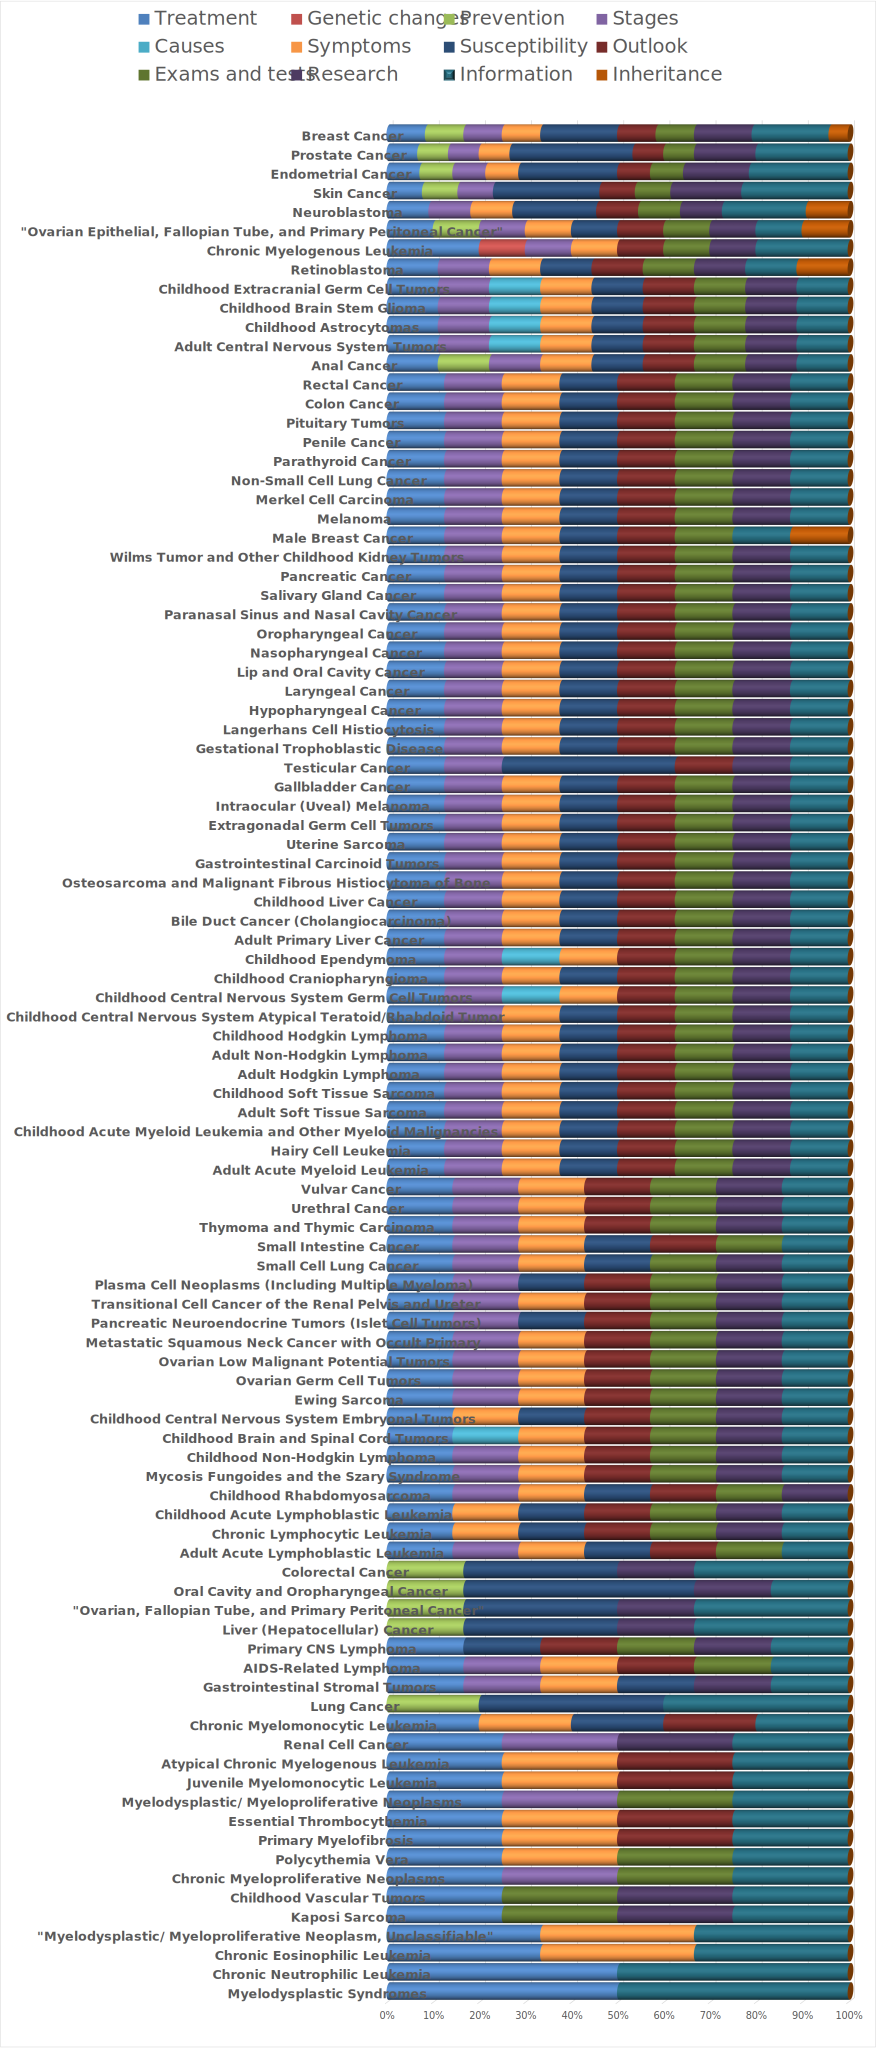
\includegraphics[scale=0.797]{Images/Cancer_qtypes.png}
	 	\caption{List of the Cancer type and question type and their count}
	 	\label{fig:cancer-type-qtype-count}
	 	\Description{A woman and a girl in white dresses sit in an open car.}
	 \end{figure}

 
 	\subsection*{Data format}
 		MedQuAD's cancer dataset are in Extensible Markup Language (XML)~\cite{MedQuAD-Cancer-dataset}, with spcific tags as shown in Table~\ref{tab:xml-tag}:
 		 	\begin{table}[ht]
 			\caption{List of the question type and their count}
 			\label{tab:xml-tag}
 			\begin{tabular}{ll}
 				\toprule
 				XML tags&Description\\
 				\midrule
 				Focus & Focus of the question\\
 				UMLS & A standardized semantic knowledge source\\
 				CUI & Concept Unique Identifier \\
 				SemanticType &  Semantic Features of questions \\
 				SemanticGroup & Semantic Group of questions\\
 				Question & The question text\\
 				Answer & The answer text\\
 				\bottomrule
 			\end{tabular}
 		\end{table}
 		
	 	For example:
	 	\begin{lstlisting}
	 		<Document id="0000001_1" source="CancerGov" url="https://www.cancer.gov/types/leukemia/patient/adult-all-treatment-pdq">
	 			<Focus>Adult Acute Lymphoblastic Leukemia</Focus>
	 			<FocusAnnotations>
 					<UMLS>
				 		<CUIs>
				 			<CUI>C0751606</CUI>
				 		</CUIs>
				 		<SemanticTypes>
				 			<SemanticType>T191</SemanticType>
				 		</SemanticTypes>
				 		<SemanticGroup>Disorders</SemanticGroup>
		 			</UMLS>
	 			</FocusAnnotations>
	 			<QAPairs>
		 			<QAPair pid="1">
			 			<Question qid="0000001_1-1" qtype="information">What is (are) Adult Acute Lymphoblastic Leukemia ?</Question>
			 			<Answer>Key Points - Adult acute lymphoblastic leukemia (ALL) is a type of cancer in which the bone marrow makes too many lymphocytes (a type of white blood cell). - Leukemia may affect red blood cells, white blood cells, and platelets. - Previous chemotherapy and exposure to radiation may increase the risk of developing ALL. - Signs and symptoms of adult ALL include fever, feeling tired, and easy bruising or bleeding. - Tests that examine the blood and bone marrow are used to detect (find) and diagnose adult ALL. ...
			 			</Answer>
	 				</QAPair>
	 			</QAPairs>
	 		</Document>
	 	\end{lstlisting}
		
		Now, by the look the data looks easy to feed into BioBERT model, however, BioBERT model requier four major components ``context'', ``question'', ``answer'', and ``start\_answer''. And the given data are missing two main parts ``context'' and ``start\_answer''. So, we have to take few manual following steps to make dataset compatible to BioBERT model.
		\begin{itemize}
			\item The give ``answer'' tags contains very big string, but the correct answer is just few lines of this text. So, we made give ``answer'' tag as ``context'' tag.
			\item Manually find the correct answer and made it as ``answer'' tag.
			\item Calculate ``start\_answer''  tag from new generated ``context'' tag
			\item finally, stored every data in JavaScript Object Notation (JSON) format.
		\end{itemize}
	
		Example of new data:
		\begin{lstlisting}
			{"data": [{
				"title": "information", 
				"paragraphs": [{
					"context": "Key Points Adult acute lymphoblastic leukemia (ALL) is a type of cancer in which the bone marrow makes too many lymphocytes (a type of white blood cell). Leukemia may affect red blood cells, white blood cells, and platelets. Previous chemotherapy and exposure to radiation may increase the risk of developing ALL. Signs and symptoms of adult ALL include fever, feeling tired, and easy bruising or bleeding. Tests that examine the blood and bone marrow are used to detect (find) and diagnose adult ALL. ...", 
					"qas": [{
						"answers": [{
							"text": "Adult acute lymphoblastic leukemia (ALL) is a type of cancer in which the bone marrow makes too many lymphocytes (a type of white blood cell).", 
							"answer_start": 11
						}], 
						"question": "What is (are) Adult Acute Lymphoblastic Leukemia ?", "id": "1"
					}]
				}],
				...}, 
				"version": "1.1", 
				"team": "nlp-group-project-fall-2020-deepbiocomp", 
				"Disease": "Cancer"
			}
		\end{lstlisting}
	
	\section*{Method}
	The following sections are categorized into three main sections, first a brief explanation on the data processing and implementation methods used to fine-tune the BioBERT model for regular question answering. Second, the data processing and fine-tuning of the GPT2 model for text-generation which is the basis for creation of long comprehensive answers. Finally, the report discusses the implementation methods for a composite model that runs the fine-tuned BioBERT for Question-Answering and uses the output of the BioBERT model as the input prompt for the GPT2 text generator for a more verbose, comprehensive answer. 
	
	\subsection*{Fine-tuning BioBERT}
		The biomedical domain texts contain a vast number of domain-specific proper nouns (e.g.  BRCA1, Leukemia) which are understood mostly by biomedical researchers. In this context the   BioBERT is already fine-tuned on PubMed abstracts (PubMed) and PubMed Central full-text articles(PMC). Further, we fine-tuned again using Cancer QA dataset, the MedQuAD. The total Cancer and question type is summarized in Figure~\ref{fig:cancer-type-qtype-count}. 
		
	\subsection*{Fine-tuning GPT2}
		This section will briefly explain the data used to pretraint the GPT2 model and how the script that was implemented to use the GPT2 model for text generation. The GPT2 model was chosen for this task because of the robustness of the model and its ability to generate long sentences while maintaining relatively good semantic sense. However, the language model is much too general and requires fine-tuning to work effectively and generative texts pertinent to cancer queries. Thus, the model was fine-tuned on the same MedQuAD dataset that was used to fine-tune the aforementioned BioBERT model.
		
		However, unlike the BioBERT model which is used for question-answering, the data must be processed differently for the GPT2 model. In the case of the question-answering models, the dataset usually has three major components, the `question', `context' and the `answer'. All of which are important for training a question-answering model, but fine-tuning a language model (GPT2) does not require all three components. Concretely, the GPT2 model was trained only using the `context' of the dataset. Furthermore,  two special tokens were added, the `<BOS>' signifying the beginning of a sentence and a `<EOS>' token, signifying the end of a sentence. The code for fine-tuning the GPT2 model is based on an older (not currently available) script from the huggingface transformer git repo called `run\_language\_modelling.py'. The script was modified and reimplemented as a jupyter notebook. Furthermore, it was also modified to let GPT2 accept the special tokens as mentioned above. Once the model was fine-tuned with our desired dataset, it was saved locally to be used for can related text-generation.
		
	\subsection*{Composite Model for Comprehensive Question Answering}
		The final section will discuss the composite model that stacks the fine-tuned GPT2 based text-generation model on top of  the fine-tuned BioBERT model for question-answering. The question-answering code is based on the `run\_squad.py' script from the Huggingface’s Transformer git repository. The fine-tuned model takes as input the question provided by the user and tries to give an answer that is correct and contextually relevant to the question asked. Once, the BioBERT model returns an answer for the given query, the output is used as the input for the GPT2 model. The text-generation code is based on the `run\_generation.py' script from the Huggingface’s Transformer git repository. The script has been heavily modified and rewritten as a python function in a jupyter notebook. It has also been modified to accept our dataset which contains the `<BOS>' and `<EOS>' special tokens. The text-generation model returns two suitable answers which are generated based on the prompt provided from the question-answering model. The resulting final answer is not only verbose and comprehensive but semantically and contextually relevant to the question asked. Thus, providing a much better experience to the user submitting the queries to the model.
	
	\section*{Results}
	This section of the report will discuss the results obtained from the two models used in this project, the metrics used to measure the accuracy of the model and the qualitative measure of the generated answers.
	
	\subsection*{Training and Accuracy Metrics}
		First, the BioBERT model was fine-tuned on our dataset. The model was trained for 20 epoch running on 4 GPU cores. The model reduced the loss value with each epoch during training. Then, the following accuracy metrics scores were achieved during evaluation on test data.
		\begin{itemize}
			\item `exact': 70.83333333333333
			\item `f1': 77.78311271345326,
			\item `total': 72,
			\item `HasAns\_exact': 70.83333333333333,
			\item `HasAns\_f1': 77.78311271345326,
			\item `HasAns\_total': 72,
			\item `best\_exact': 70.83333333333333,
			\item `best\_exact\_thresh': 0.0,
			\item `best\_f1': 77.78311271345326,
			\item `best\_f1\_thresh': 0.0
		\end{itemize}
		The accuracy metrics were monitored carefully to ensure that the model generalizes well and not overfit to the training data.
		
		Next, the GPT2 model was fine-tuned on the data processed for it. This model was tuned for 19 epochs and the loss value decreased with each epoch. Once the model was tuned,  the accuracy of the model was evaluated on the text data. The primary metric used was the perplexity score of the model which is as follows,
		\begin{itemize}
			\item `perplexity': 2.5901412982272793.
		\end{itemize} 
		Again, special attention is given to ensure that the model remains general and not overfit to the data. 
		
	\subsection*{Qualitative Results}
		Given the nature of the project, numeric accuracy scores may not be an intuitive indicator of the performance of the model. Thus, a few examples are given below that shows the question asked to the model, the answer given by the BioBERT model and the verbose, comprehensive answer given by the GPT2 model stacked on top.
		
		\begin{enumerate}
			\item[Set 1:]\qquad\\
				\textbf{Question}: ``What are the symptoms of ovarian rian Germ Cell Tumors ?''
				
				\textbf{Answer}: signs of ovarian germ cell tumor are swelling of the abdomen or vaginal bleeding after menopause.
				
				\textbf{Comprehensive}: 
					\begin{itemize}
						\item \textbf{Answer 1}: signs of ovarian germ cell tumor are swelling of the abdomen or vaginal bleeding after menopause. These and other signs and symptoms may be caused by ovarian germ cell tumor or by other conditions. Check with your doctor if you have any of the following: Weakness or feeling tired. Weight loss with little or no effect on menstrual periods. Vaginal bleeding after menopause. Sometimes pain or swelling in a women's vagina. Fever or night sweats.
						
						\item \textbf{Answer 2}: signs of ovarian germ cell tumor are swelling of the abdomen or vaginal bleeding after menopause. These and other signs and symptoms may be caused by ovarian germ cell tumor or by other conditions. Check with your doctor if you have any of the following: Swelling of the abdomen or vaginal bleeding after menopause. Trouble starting the flow of urine. Weight loss for no known reason. Trouble emptying the bladder completely after menopause. Pain or feeling of fullness below the ribs on the left side. Fever for no known reason. Easy bruising or bleeding. Pain or feeling of fullness below the ribs on the right side.
						
						\item \textbf{Answer 3}: signs of ovarian germ cell tumor are swelling of the abdomen or vaginal bleeding after menopause. Other conditions can increase the risk of hairy cell leukemia. Check with your doctor if you have any of the following: Pain or swelling in the abdomen. Weakness or feeling tired. Weight loss for no known reason. A menstrual period that does not go away.
						
						\item \textbf{Answer 4}: signs of ovarian germ cell tumor are swelling of the abdomen or vaginal bleeding after menopause. These and other signs may be caused by ovarian germ cell tumor or by other conditions. Check with your doctor if you have any of the following: Pain or swelling in the abdomen. A lump in the abdomen, vagina, or rectum. Weight loss for no known reason. Pain or a feeling of fullness below the ribs on the left side. Weight loss with no known reason. A dark urine like color that does not go away.
					\end{itemize}	
			\item[Set 2:]\qquad\\
				\textbf{Question}: ``What are the stages of Vulvar Cancer  ?''
				
				\textbf{Answer}: stage i stage ii stage iii stage iv after vulvar cancer has been diagnosed, tests are done to find out if cancer cells have spread within the vulva or to other parts of the body.
				
				\textbf{Comprehensive}: 
				\begin{itemize}
					\item \textbf{Answer 1}: stage i stage ii stage iii stage iv after vulvar cancer has been diagnosed, tests are done to find out if cancer cells have spread within the vulva or to other parts of the body. Cancer that has spread within the vulva to other parts of the body is called seminoma. A biopsy is done to diagnose seminoma. A biopsy is done during surgery to remove the tumor. Sometimes, a small incision (cut) is made in the vulva and a laparoscope (a thin, lighted tube) is inserted into it. The doctor will usually remove the tumor and a small amount of tissue, after the doctor has removed all the cancer. The tissue sample is checked under a microscope for signs of cancer. A pathologist views the tissue under a microscope to look for cancer cells. If cancer cells are not found, it may not be necessary to remove more tissue. There are three ways that cancer spreads in the body. Cancer can spread through tissue, the lymph system, and the blood: Tissue. The cancer spreads from where it began by growing into nearby areas. Lymph system. The cancer spreads from where it began by getting into the lymph system. The cancer travels through the lymph vessels to other parts of the body. Blood. The cancer spreads from where it began by getting into the blood. The cancer travels through the blood vessels to other parts of the body. Cancer may spread from where it began to other parts of the body through organs and tissues. When cancer spreads to another part of the body, it is called metastasis. Cancer cells break away from where they began (the primary tumor) and travel through the lymph system or blood.
					
					\item \textbf{Answer 2}: stage i stage ii stage iii stage iv after vulvar cancer has been diagnosed, tests are done to find out if cancer cells have spread within the vulva or to other parts of the body. The following stages are used for vulvar cancer: Stage I Stage II Stage III Stage IV Stage V After vulvar cancer has been diagnosed, tests are done to find out if cancer cells have spread within the vulva or to other parts of the body. The process used to find out if cancer has spread within the vulva or to other parts of the body is called staging. The information gathered from the staging process determines the stage of the disease. It is important to know the stage in order to plan treatment. Vulvar cancer in men may affect the risk of developing rectal cancer. Having rectal cancer during surgery can increase the risk of rectal cancer and is called a risk factor. Having rectal cancer in a first degree relative (parent, brother, or sister) increases the risk even more.
				\end{itemize}	
		\end{enumerate}
	
	
	\section*{Conclusion}
	The answers or responses produced by our fine-tuned model support the relevance of the question in logic with cancer QA. Our model also highlights the effectiveness of combining text generative and long-former models for further model improvement. Our findings also show that relying on a restricted set of reliable answer sources can bring a plentiful improvement in domain-specific QA.
	
	\subsection*{Future Plans}
		The dataset used in this project has on average a very long context paragraph. For the ease of fine-tune on available resources, the only initial part of the context was used. Further, the transformer-based models like BioBERT are inefficient to handle long sequences due to expensive self-attention operations. To address this limitation, we will fine-tune the Longformer. As compared to the BioBERT (transformer-based), the attention mechanism in the Longformer scales linearly with sequence length. This feature helps it to process medical documents of thousands of tokens or longer. 
		Additionally, the chosen dataset (transformer-based) is too small and we were unable to procure the dataset from BoiASK. When available we will finetune over this big data set to add more diversity to the model.
	
	\bibliographystyle{ACM-Reference-Format}
	\bibliography{ref}
	
\end{document}